\documentclass[11pt,letterpaper]{article}
\usepackage[T1]{fontenc}
\usepackage[utf8]{inputenc}
\usepackage{lmodern}
\usepackage[margin=0.9in,headheight=15pt,headsep=18pt]{geometry}
\usepackage{amsmath,amssymb,mathtools,mathrsfs}
\usepackage{microtype}
\usepackage{booktabs,longtable,array}
\usepackage{graphicx}
\usepackage[section]{placeins}
\usepackage{xcolor}
\usepackage{enumitem}
\usepackage{fancyhdr}
\usepackage{titlesec}
\usepackage{tocloft}
\setlength{\cftbeforesecskip}{3pt}
\renewcommand{\cftsecfont}{\small}
\renewcommand{\cftsecpagefont}{\small}
\usepackage{needspace}
\usepackage{xurl}
\usepackage{hyperref}
\hypersetup{hidelinks,pdftitle={Komorebi Large Signal Model: Visual Atlas 1.0.0},pdfauthor={Komorebi P.}}
\setlength{\parindent}{0pt}
\setlength{\parskip}{0.52em}
\setlength{\emergencystretch}{2em}
\setcounter{secnumdepth}{-1}
\setcounter{tocdepth}{1}
\titleformat{\section}{\Large\bfseries}{\thesection}{0em}{}
\titlespacing*{\section}{0pt}{1.7em}{0.7em}
\titleformat{\subsection}{\large\bfseries}{\thesubsection}{0em}{}
\titlespacing*{\subsection}{0pt}{1.15em}{0.5em}
\clubpenalty=10000
\widowpenalty=10000
\displaywidowpenalty=10000
\allowdisplaybreaks[1]
\providecommand{\tightlist}{\setlength{\itemsep}{0pt}\setlength{\parskip}{0pt}}
\providecommand{\passthrough}[1]{#1}
\pagestyle{fancy}
\fancyhf{}
\fancyhead[L]{\small\textsc{Komorebi Large Signal Model}}
\fancyhead[R]{\small Foundations 1.0.0}
\fancyfoot[L]{\small Komorebi P.}
\fancyfoot[R]{\small\thepage}
\renewcommand{\headrulewidth}{0.3pt}
\begin{document}
\hypersetup{pageanchor=false}
\begin{titlepage}
\vspace*{0.5in}
{\small\textsc{Operation Komorebi}\par}
\vspace{0.72in}
{\fontsize{33}{39}\selectfont\bfseries Large Signal Model\par}
\vspace{0.3in}
{\fontsize{21}{27}\selectfont A visual atlas of the finite foundations\par}
\vspace{0.45in}
\rule{\textwidth}{0.45pt}\par
\vspace{0.3in}
\begin{minipage}{0.95\textwidth}
\large
Thirteen preserved mathematical illustrations.\\State, transfer, probability and evidence.\\No new empirical performance claims.
\end{minipage}
\vfill
{\Large Komorebi P.\par}
\vspace{0.2in}
{\normalsize Foundations 1.0.0: frozen finite theory release\par}
{\normalsize Companion to PR-LASM software release 2.3.0\par}
{\normalsize 10 October 2026\par}
\end{titlepage}
\hypersetup{pageanchor=true}
\begingroup\footnotesize\setlength{\cftbeforesecskip}{0pt}\tableofcontents\endgroup\bigskip

\section{Visual atlas of the finite
foundations}\label{visual-atlas-of-the-finite-foundations}

\textbf{Foundations 1.0.0. Thirteen preserved mathematical
illustrations.}

This atlas follows the argument from observable state and packet
interactions to admissible probability domains, continuous observations,
repair and dependent-data confidence. Every plot is an unchanged
Python-generated asset from the earlier foundations blocks. No new
experiment, score or learned checkpoint is introduced.

Read the associated proposition and its setup before applying an
illustrated result. Curves are finite calculations, certificate geometry
or proved upper bounds as stated. A figure is not a proof of a
quantified theorem. The source-identity ledger is
\path{VISUAL_ATLAS_SOURCES.json}.

\newpage

\section{1. A history can carry the missing
state}\label{a-history-can-carry-the-missing-state}

\textbf{Theory:} P14--17, P25.

\begin{center}
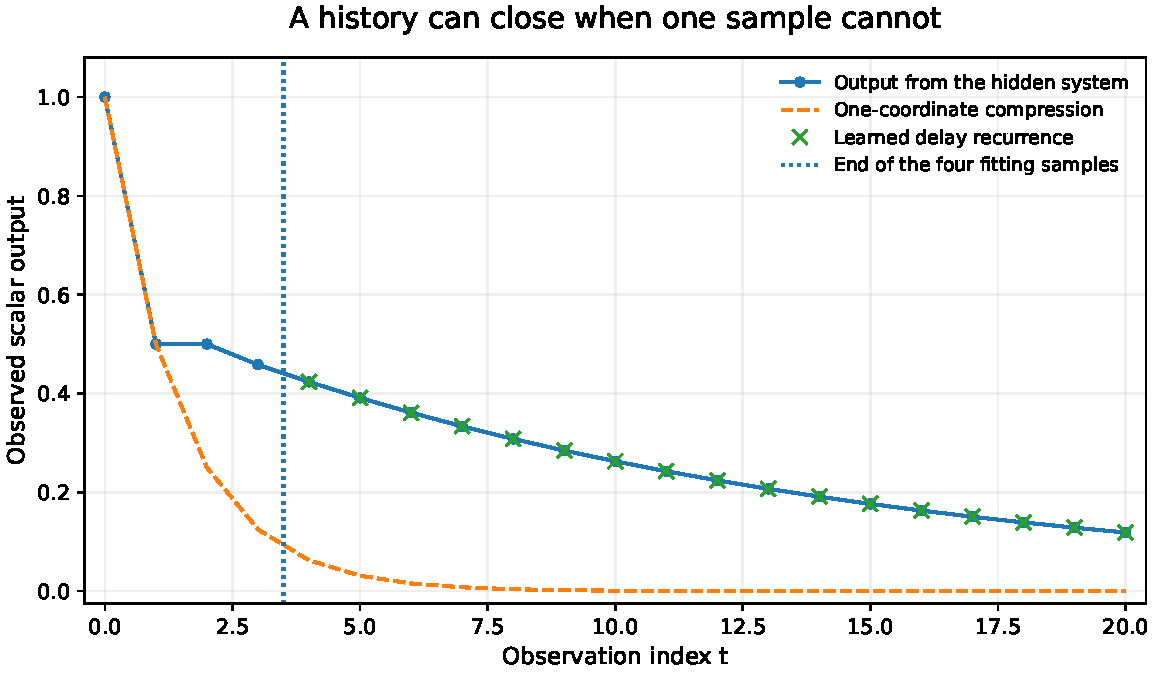
\includegraphics[width=\linewidth,height=0.51\textheight,keepaspectratio]{../figures/01_delay_prediction.pdf}
\end{center}

One scalar sample need not determine the next sample. A sufficiently
long history can close under a declared finite linear model. The plotted
delay realization uses the same output-only example as the cumulative
volume. The vertical line separates the four fitting samples from
continuation.

\textbf{Boundary.} The matching continuation is a finite example. Full
identification depends on rank, delay closure and coverage, not on the
appearance of these curves.

\textbf{Preserved asset:} \path{01_delay_prediction.pdf}.

\newpage

\section{2. Retain memory or enlarge the
state}\label{retain-memory-or-enlarge-the-state}

\textbf{Theory:} P10, P18--19.

\begin{center}
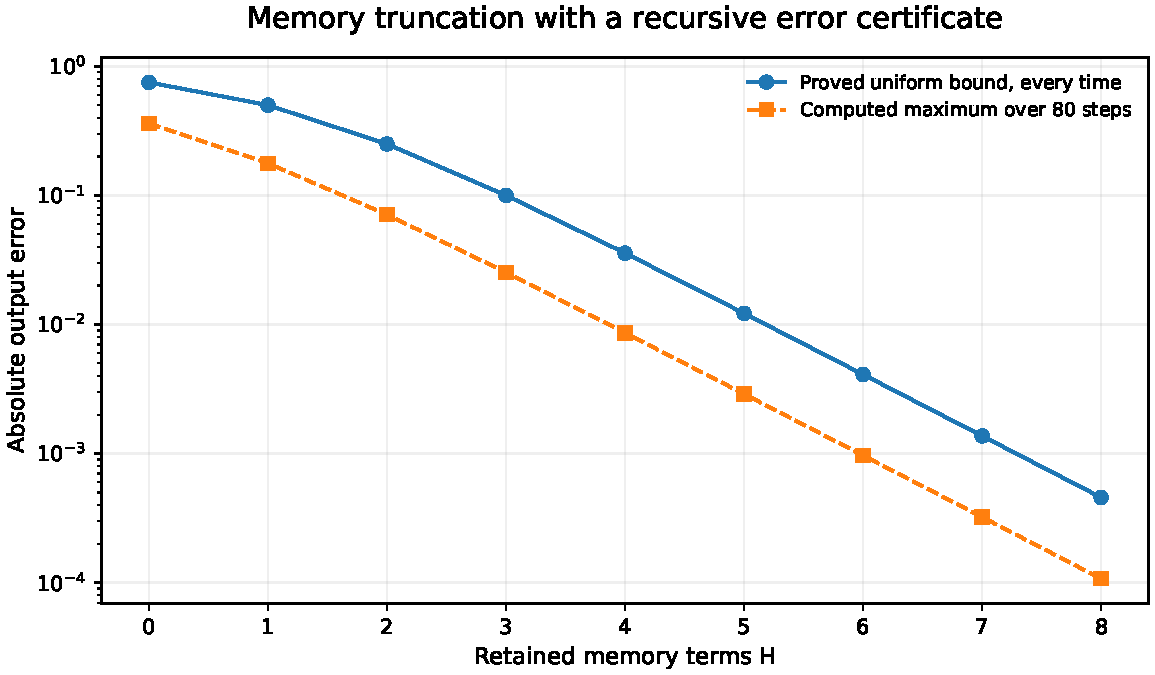
\includegraphics[width=\linewidth,height=0.51\textheight,keepaspectratio]{../figures/02_memory_certificate.pdf}
\end{center}

Eliminating unresolved coordinates creates an exact memory kernel.
Truncating that kernel changes the dynamics. Under the stated
contraction condition, the recursive prediction error has a computable
upper bound. The plotted finite error and the bound are different
quantities.

\textbf{Boundary.} The maximum computed over 80 steps does not establish
the all-time statement. The written contraction argument supplies that
statement under its hypotheses.

\textbf{Preserved asset:} \path{02_memory_certificate.pdf}.

\newpage

\section{3. Small omitted energy is not small
influence}\label{small-omitted-energy-is-not-small-influence}

\textbf{Theory:} P5, P7, P20.

\begin{center}
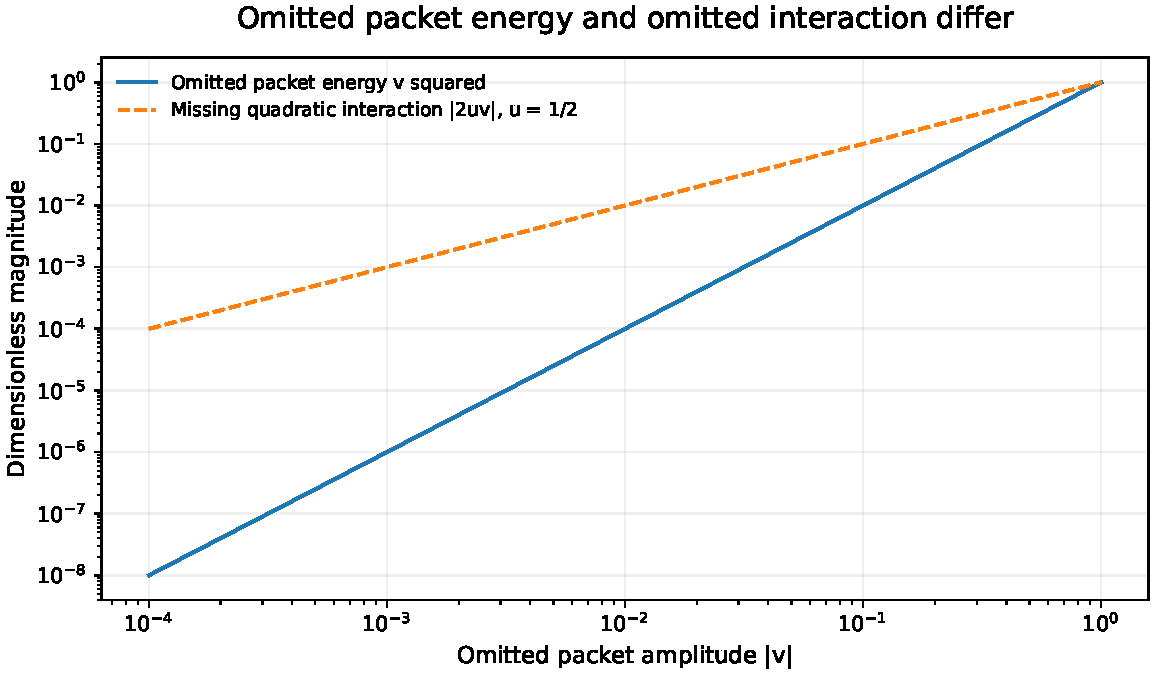
\includegraphics[width=\linewidth,height=0.51\textheight,keepaspectratio]{../figures/06_packet_interaction.pdf}
\end{center}

A nonlinear operation couples packets. For a square, the mixed term is
proportional to the omitted amplitude while its energy is quadratic in
that amplitude. The plot keeps those two scales visible. Refinement must
account for transfer or interaction, not only reconstruction energy.

\textbf{Boundary.} A packet decomposition is not a collection of
independent nonlinear subsystems. Dropping interaction terms requires
its own approximation budget.

\textbf{Preserved asset:} \path{06_packet_interaction.pdf}.

\newpage

\section{4. A finite witness for all future
branches}\label{a-finite-witness-for-all-future-branches}

\textbf{Theory:} P39, P45, P49.

\begin{center}
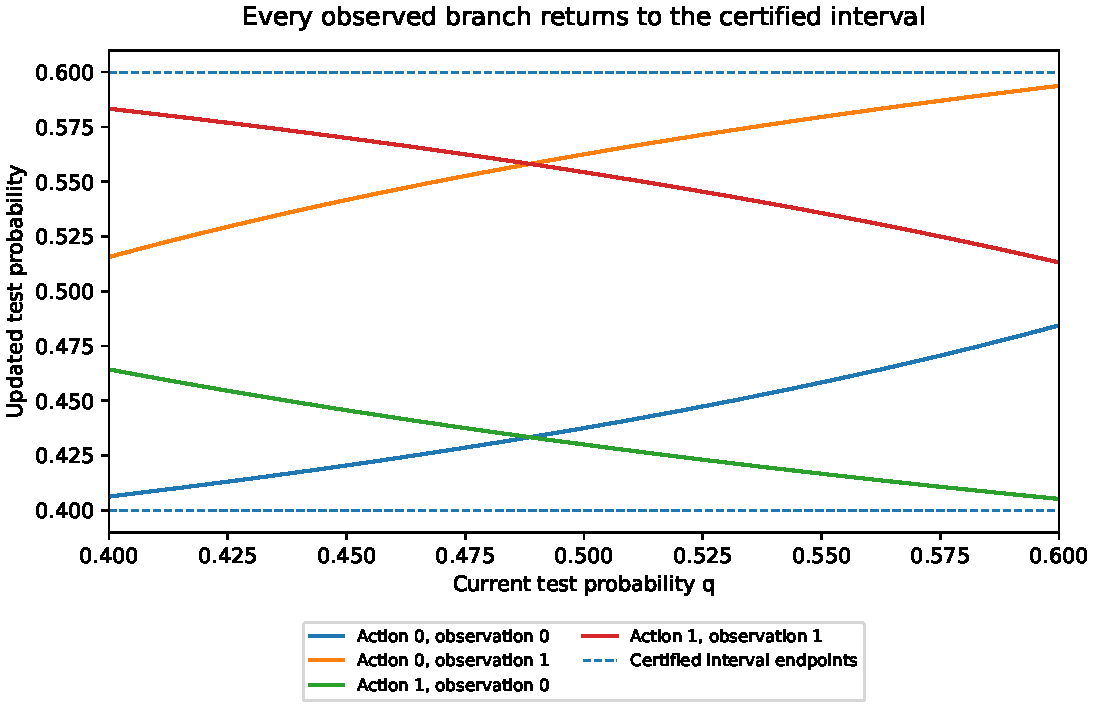
\includegraphics[width=\linewidth,height=0.51\textheight,keepaspectratio]{../figures/14_certified_interval.pdf}
\end{center}

The fitted two-coordinate model maps every branch back into the interval
from 2/5 to 3/5. Its exact positive-lift witness checks generators,
nonnegative branch matrices, mass conservation and the initial weights.
The plotted maps illustrate the same certified interval.

\textbf{Boundary.} The plotted grid is not the all-horizon proof.
Intertwining and nonnegativity establish validity of the submitted
model. They do not establish that it is the true process.

\textbf{Preserved asset:} \path{14_certified_interval.pdf}.

\newpage

\section{5. A small state may need a curved
domain}\label{a-small-state-may-need-a-curved-domain}

\textbf{Theory:} P46--47.

\begin{center}
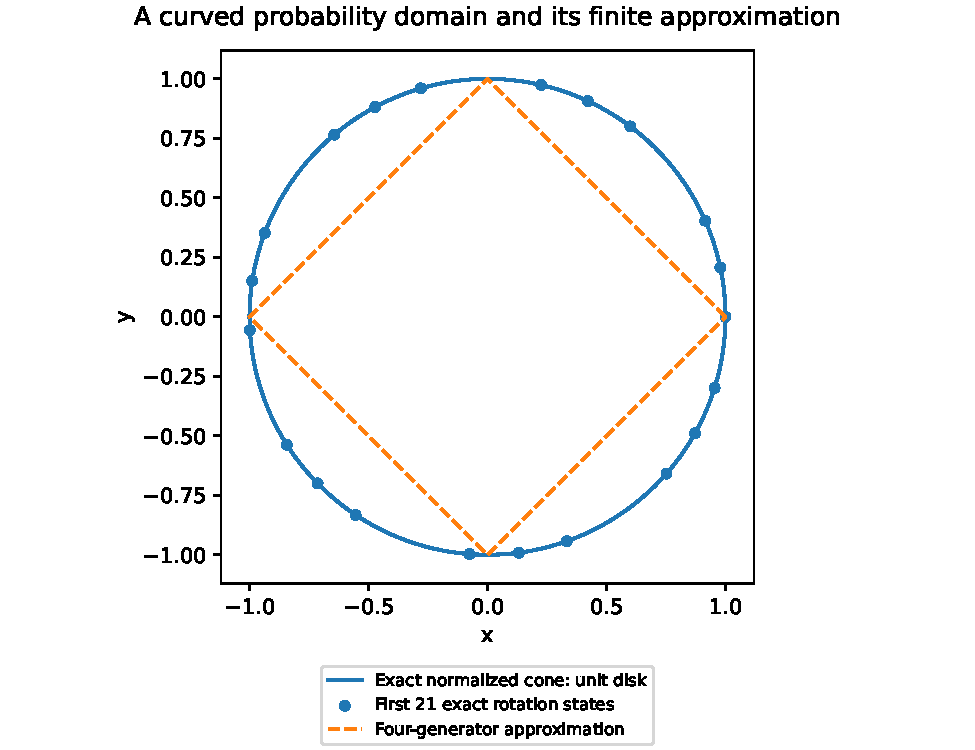
\includegraphics[width=\linewidth,height=0.51\textheight,keepaspectratio]{../figures/18_curved_probability_domain.pdf}
\end{center}

The rational rotation example has a three-coordinate realization whose
normalized probability domain is the disk. The displayed orbit is
finite, while the proof establishes density and rules out an exact
finite polyhedral domain for this model.

\textbf{Boundary.} The inscribed diamond becomes useful only after a
declared modification of the dynamics. Replacing the disk by a finite
picture is not exact state refinement.

\textbf{Preserved asset:} \path{18_curved_probability_domain.pdf}.

\newpage

\section{6. A curved domain can have a finite
certificate}\label{a-curved-domain-can-have-a-finite-certificate}

\textbf{Theory:} P50--53.

\begin{center}
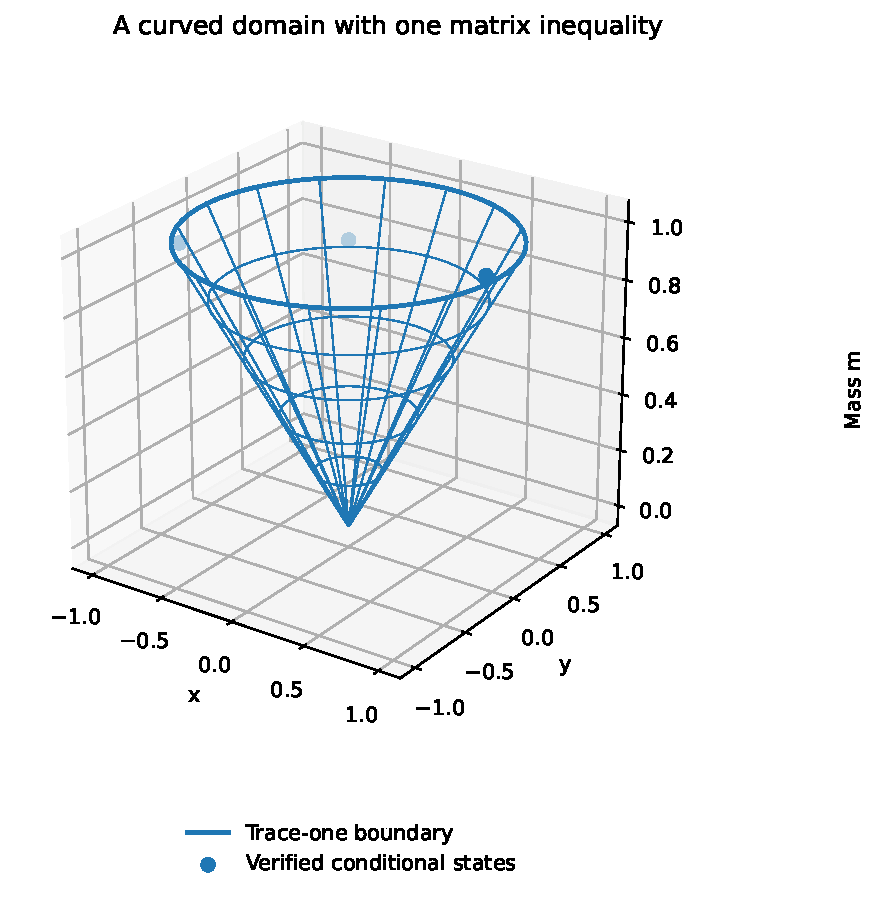
\includegraphics[width=\linewidth,height=0.51\textheight,keepaspectratio]{../figures/21_matrix_probability_cone.pdf}
\end{center}

The Lorentz cone admits a two-by-two positive-semidefinite matrix
representation. Congruence identities certify the unchanged rotation and
observation operations. This resolves the certificate-language
limitation without damping the exact model.

\textbf{Boundary.} The matrix representation is a mathematical
positivity witness. No quantum hardware, physical quantum process or
quantum advantage is asserted.

\textbf{Preserved asset:} \path{21_matrix_probability_cone.pdf}.

\newpage

\section{7. Averaging and quadratic action do not
commute}\label{averaging-and-quadratic-action-do-not-commute}

\textbf{Theory:} P56--59.

\begin{center}
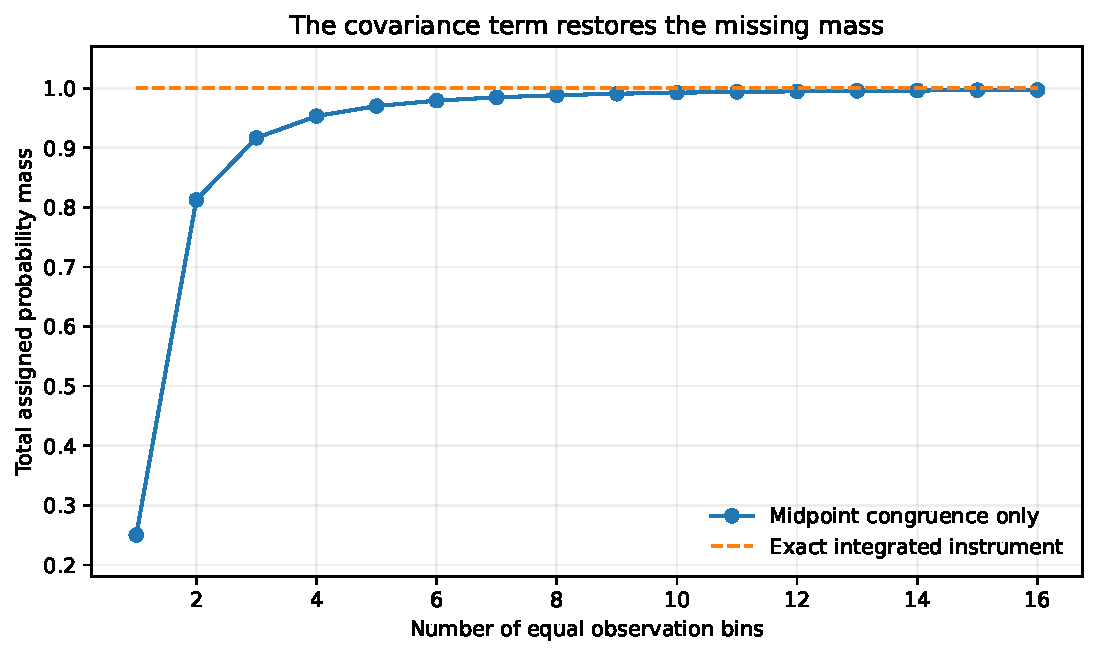
\includegraphics[width=\linewidth,height=0.51\textheight,keepaspectratio]{../figures/26_binning_mass_defect.pdf}
\end{center}

Midpoint congruences omit a covariance contribution. For this worked
model, using n equal observation bins loses mass 3/(4n²). Exact
integration retains the missing term and preserves normalization. At one
bin the naive approximation retains only one quarter of total mass.

\textbf{Boundary.} Event coarsening is exact for the stated bin-based
policy. A policy that responds to values within a bin is a different
comparison.

\textbf{Preserved asset:} \path{26_binning_mass_defect.pdf}.

\newpage

\section{8. Proposal and certificate are separate
stages}\label{proposal-and-certificate-are-separate-stages}

\textbf{Theory:} P62--63.

\begin{center}
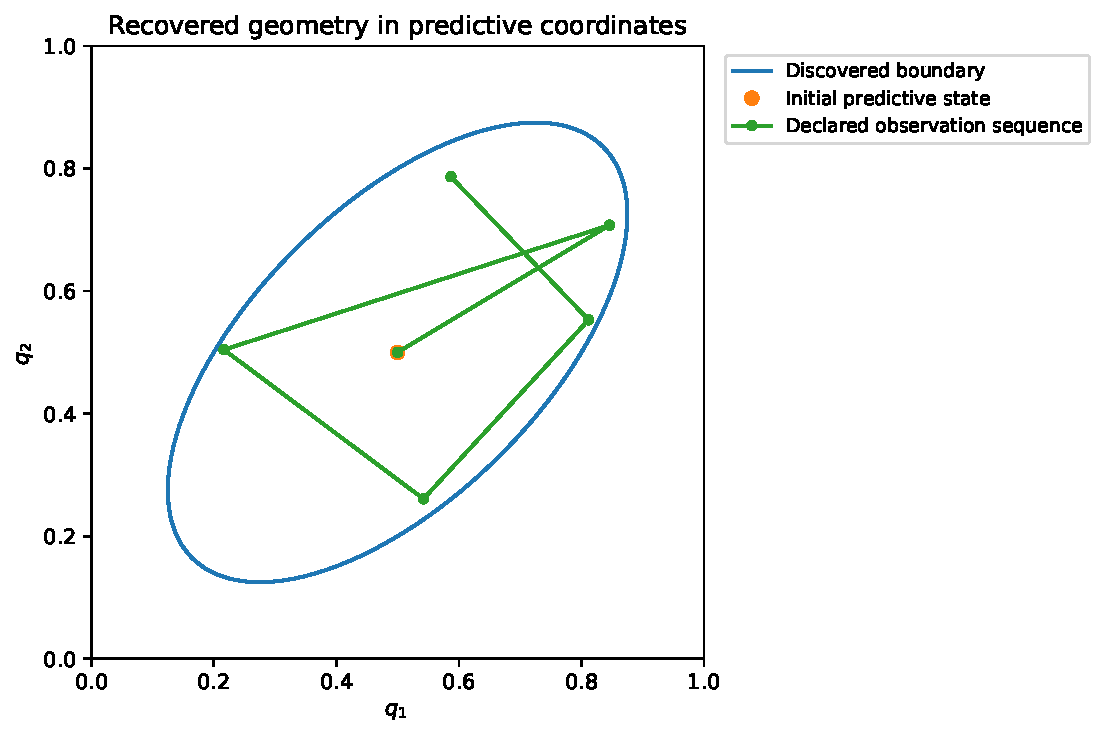
\includegraphics[width=\linewidth,height=0.51\textheight,keepaspectratio]{../figures/28_discovered_geometry.pdf}
\end{center}

The exact example constructs an ellipse from observable operators,
rather than taking its metric from a supplied template. The trajectory
remains in the discovered domain. The accepted witness independently
checks every operator, orientation and initial state.

\textbf{Boundary.} This is restricted exact invariant-form discovery,
not general discovery of hidden state or noisy geometry from arbitrary
observations.

\textbf{Preserved asset:} \path{28_discovered_geometry.pdf}.

\newpage

\section{9. Conditional tests can expose a missed
dependence}\label{conditional-tests-can-expose-a-missed-dependence}

\textbf{Theory:} P66--70.

\begin{center}
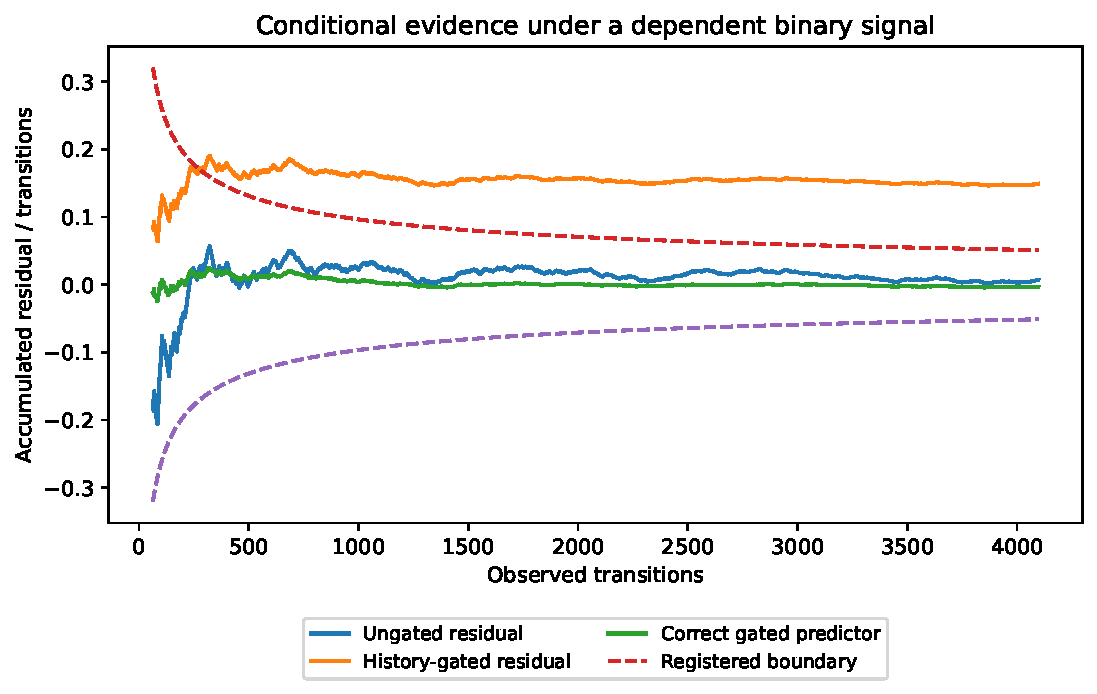
\includegraphics[width=\linewidth,height=0.51\textheight,keepaspectratio]{../figures/32_dependent_evidence.pdf}
\end{center}

An ungated average can look compatible with a constant predictor while a
prospectively chosen history-gated test reveals conditional mismatch.
The figure uses the saved seeded path and its registered time-uniform
boundary.

\textbf{Boundary.} It is one illustrative dependent path, not an
empirical coverage study. Rejection can certify a lower discrepancy.
Nonrejection is not an upper accuracy guarantee.

\textbf{Preserved asset:} \path{32_dependent_evidence.pdf}.

\newpage

\section{10. Validity repair has a measurable
cost}\label{validity-repair-has-a-measurable-cost}

\textbf{Theory:} P73, P79--80.

\begin{center}
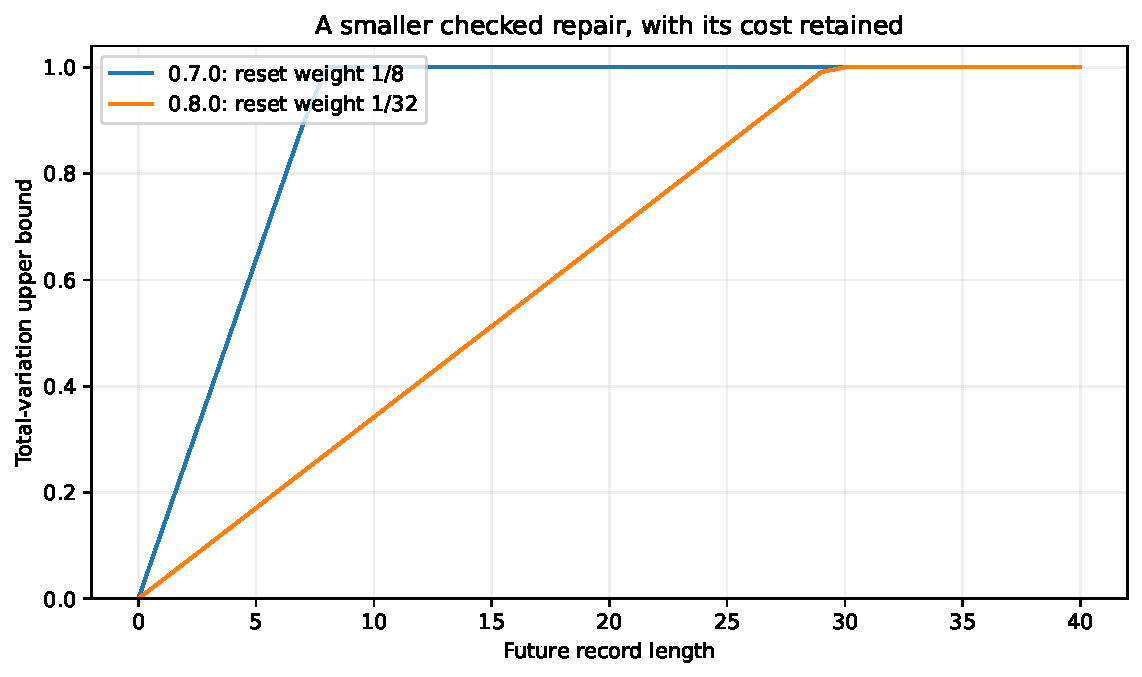
\includegraphics[width=\linewidth,height=0.51\textheight,keepaspectratio]{../figures/41_smaller_repair.pdf}
\end{center}

The same proposed geometry and perturbed operator family are certified
with reset weight 1/32 instead of 1/8. The retained uncertainty radius
is unchanged. The newer conservative full-record bound first becomes
trivial at horizon 30 rather than eight.

\textbf{Boundary.} These lines are upper bounds, not observed model
errors. The smaller repair is bracketed for one fixed geometry and reset
path, not globally optimized.

\textbf{Preserved asset:} \path{41_smaller_repair.pdf}.

\newpage

\section{11. Learned coefficients need declared
observations}\label{learned-coefficients-need-declared-observations}

\textbf{Theory:} P81--84, P87.

\begin{center}
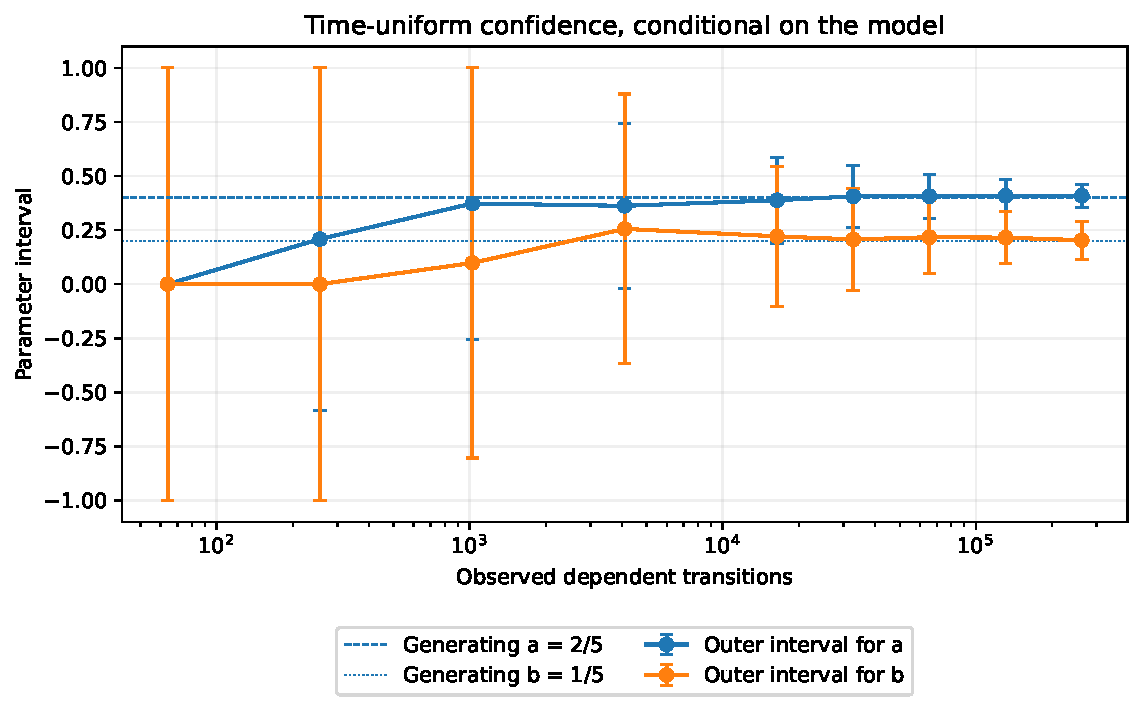
\includegraphics[width=\linewidth,height=0.51\textheight,keepaspectratio]{../figures/42_confidence_intervals.pdf}
\end{center}

The intervals are from the saved five-node dependent path. The state
map, two-parameter family, reference measure and predictable protocol
are supplied. The learner estimates two parameters and rounds its
intervals outward.

\textbf{Boundary.} The confidence guarantee is conditional and
simultaneous over time. One saved path does not validate coverage
empirically or authenticate the model assumptions.

\textbf{Preserved asset:} \path{42_confidence_intervals.pdf}.

\newpage

\section{12. Structured uncertainty can preserve a boundary
ray}\label{structured-uncertainty-can-preserve-a-boundary-ray}

\textbf{Theory:} P83, P87.

\begin{center}
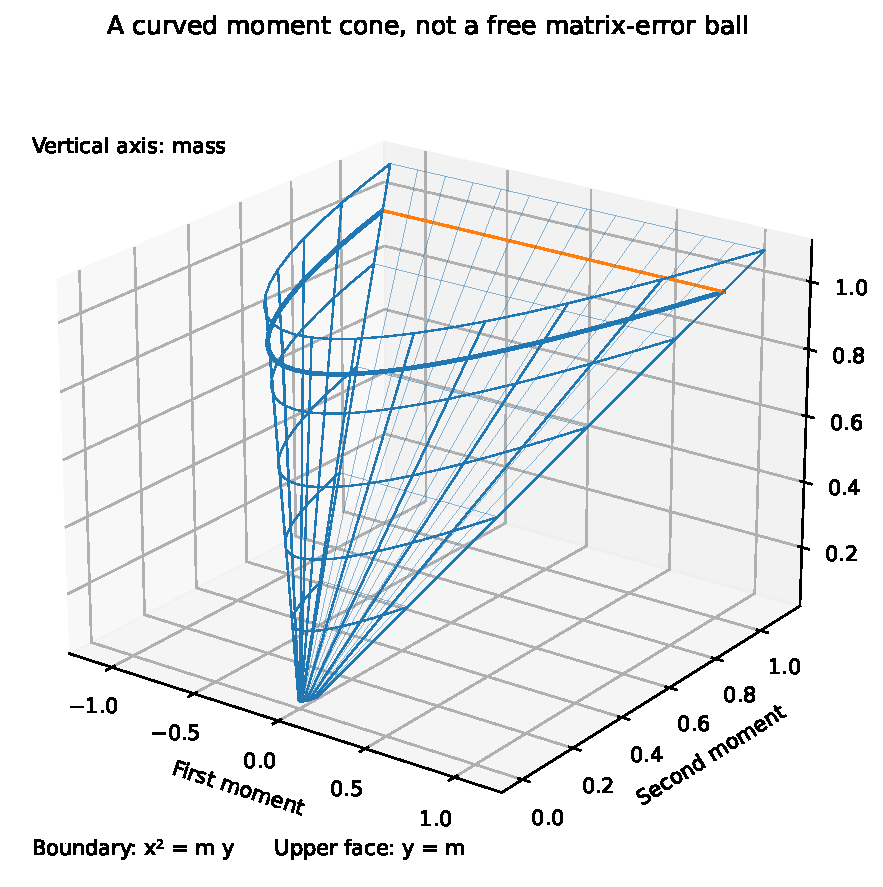
\includegraphics[width=\linewidth,height=0.51\textheight,keepaspectratio]{../figures/44_moment_cone.pdf}
\end{center}

The moment cone is defined by a positive-semidefinite two-by-two moment
matrix and an upper second-moment constraint. Parameter uncertainty
changes the observation density but leaves the posterior state
v(u)=(1,u,u²) unchanged.

\textbf{Boundary.} This structured parameter family is not a free
matrix-entry uncertainty ball. The geometry and feature dictionary are
declared, not discovered by this example.

\textbf{Preserved asset:} \path{44_moment_cone.pdf}.

\newpage

\section{13. Choose the guarantee that matches the
question}\label{choose-the-guarantee-that-matches-the-question}

\textbf{Theory:} P85--87.

\begin{center}
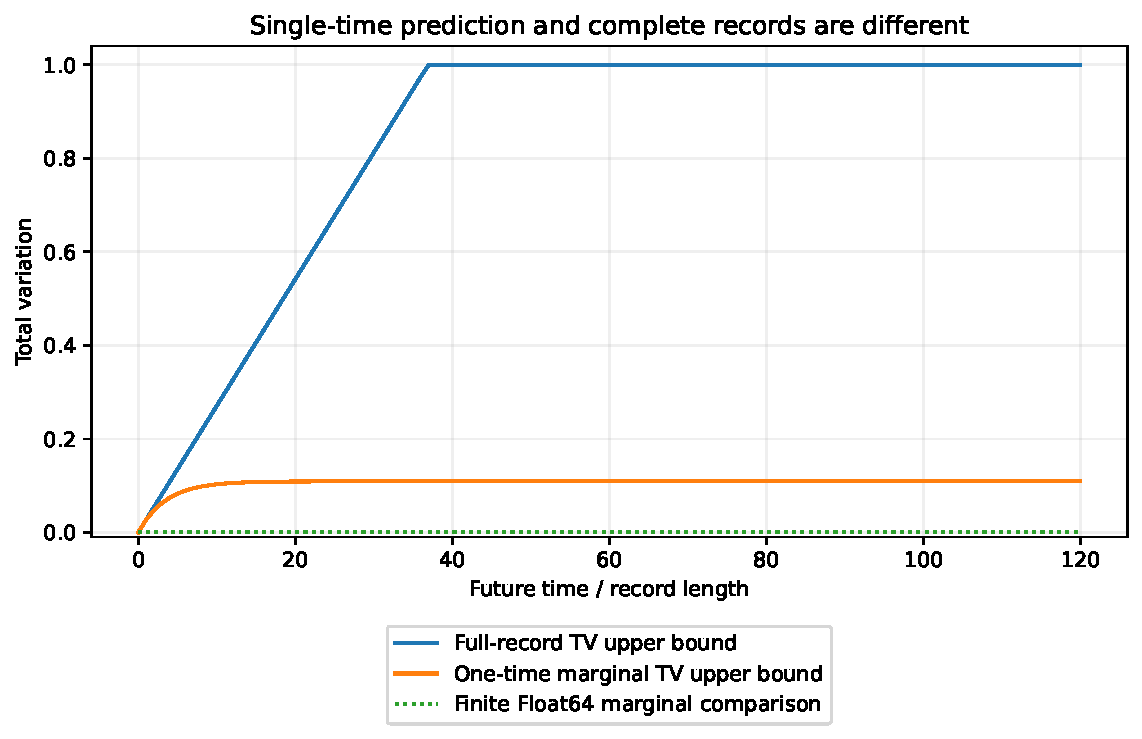
\includegraphics[width=\linewidth,height=0.51\textheight,keepaspectratio]{../figures/45_prediction_horizons.pdf}
\end{center}

The full-record bound grows with record length. The one-time marginal
bound remains uniformly informative only because the declared Markov
family has a common minorization. The figure also shows a finite
numerical marginal comparison, separately from either theorem.

\textbf{Boundary.} An all-time single-marginal bound is not an all-time
complete-record bound. Common reference measure, model class, initial
state and policy remain part of the comparison.

\textbf{Preserved asset:} \path{45_prediction_horizons.pdf}.
\end{document}
